\subsection{Component Identification in Figure T-2}
\label{T6C09}

\begin{tcolorbox}[colback=gray!10!white,colframe=black!75!black,title=T6C09]
What is component 4 in figure T-2?

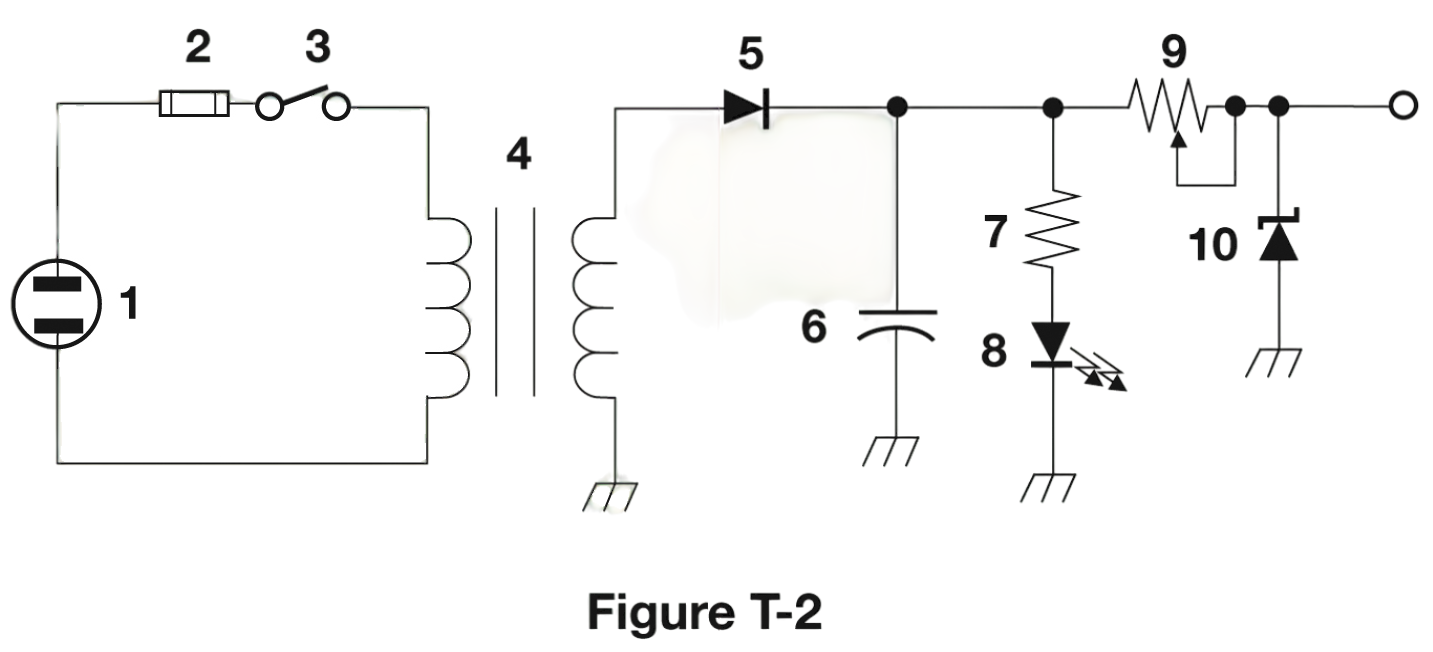
\includegraphics[width=0.5\textwidth]{tech/images/t2.png} 

\begin{enumerate}[label=\Alph*)]
    \item Variable inductor
    \item Double-pole switch
    \item Potentiometer
    \item \textbf{Transformer}
\end{enumerate}
\end{tcolorbox}

\subsubsection{Intuitive Explanation}
Imagine you have a magic box that can change the amount of electricity flowing through it. This magic box doesn’t just change the amount; it can make it higher or lower depending on what you need. That’s exactly what a transformer does! In figure T-2, component 4 is this magic box, also known as a transformer. It’s like a superhero for electricity, making sure it’s just the right strength for whatever job it needs to do.

\subsubsection{Advanced Explanation}
A transformer is an electrical device that transfers electrical energy between two or more circuits through electromagnetic induction. It consists of two coils, known as the primary and secondary windings, which are usually wound around a common magnetic core. The primary winding is connected to the input voltage, and the secondary winding delivers the transformed voltage to the load. The voltage transformation is governed by the equation:

\[
\frac{V_p}{V_s} = \frac{N_p}{N_s}
\]

where \( V_p \) and \( V_s \) are the primary and secondary voltages, and \( N_p \) and \( N_s \) are the number of turns in the primary and secondary windings, respectively. Transformers are essential in power distribution systems for stepping up or stepping down voltages to minimize energy loss during transmission.

% Prompt for generating a diagram: A diagram showing a transformer with labeled primary and secondary windings, and the magnetic core.